% !TEX root = ../main.tex

\chapter{Combinatoire des mots}\label{chap8}

\section{Exercice 20 - Coloriage non répétitif}

\subsection{$\pi(P_n)$}
Soit $\pi(P_n)$ le nombre de Thue du graphe $P_n$ c-à-d le plus petit nombre de couleurs nécessaires pour colorier la chaîne à $n$ sommets de manière non-répétitive.

Voici les graphes $P_2$, $P_3$ et $P_4$ ainsi que leur nombre de Thue.

\begin{figure}[h]
	\begin{center}
		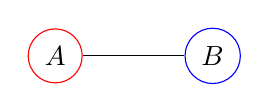
\begin{tikzpicture}
			\tikzset{node/.style={circle, draw=black}};
			\node[node,draw=red] (A) at (0,0) {$A$};
			\node[node,draw=blue] (B) at (2,0) {$B$};

			\draw[black] (A) -- (B);
		\end{tikzpicture}
	\end{center}
	\caption{$\pi(P_2)=2$}
\end{figure}

\begin{figure}[h]
	\begin{center}
		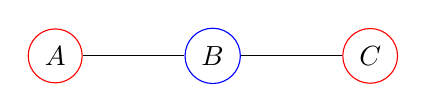
\begin{tikzpicture}
			\tikzset{node/.style={circle, draw=black}};
			\node[node,draw=red] (A) at (0,0) {$A$};
			\node[node,draw=blue] (B) at (2,0) {$B$};
			\node[node,draw=red] (C) at (4,0) {$C$};

			\draw[black] (A) -- (B) -- (C);
		\end{tikzpicture}
	\end{center}
	\caption{$\pi(P_3)=2$}
\end{figure}

\begin{figure}[h]
	\begin{center}
		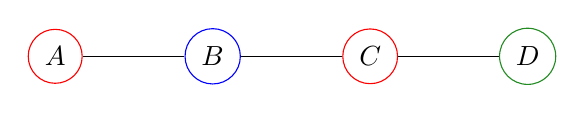
\begin{tikzpicture}
			\tikzset{node/.style={circle, draw=black}};
			\node[node,draw=red] (A) at (0,0) {$A$};
			\node[node,draw=blue] (B) at (2,0) {$B$};
			\node[node,draw=red] (C) at (4,0) {$C$};
			\node[node,draw=ForestGreen] (D) at (6,0) {$D$};

			\draw[black] (A) -- (B) -- (C) -- (D);
		\end{tikzpicture}
	\end{center}
	\caption{$\pi(P_4)=3$}
\end{figure}

Soit $H(n)$ l'hypothèse suivante : $\pi(P_n) \geq 3$. Montrons par récurrence que $H(n)$ est vraie pour tout $n \geq 4$.

D'après la figure du graphe $P_4$ ci-dessus, on a $H(4)$ vraie. On peut donc initialiser la récurrence à $n=4$.

Supposons que $H(n)$ est vraie et penchons-nous sur le graphe $P_{n+1}$. Le graphe $P_{n+1}$ étant la chaîne à $n+1$ sommets, on peut colorier une sous-chaîne de $P_n$ à $n$ sommets avec 3 couleurs ou plus de manière non-répétitive d'après l'hypothèse de récurrence. En coloriant le sommet restant avec une nouvelle couleur, on obtient donc un coloriage non-répétitif à 4 couleurs ou plus donc on a bien $H(n+1)$ vraie.

On vient de prouver que $H(n) \rightarrow H(n+1)$ donc on a bien $\pi(P_n) \geq 3, \forall n \geq 4$.


\subsection{Mot $\omega$ sans chevauchement}
Montrons que pour tout mot fini $\omega$ sur $\{a,b\}$, $\omega$ est sans chevauchement si et seulement si $\mu(\omega)$ est sans chevauchement.

Tout d'abord, supposons (sans perte de généralité) que $\omega = mno$ avec $m,n,o$ des mots sur $\{a,b\}$ qui peuvent être le mot vide. Supposons que $n = \alpha u \alpha u \alpha$ avec $\alpha$ une lettre et $u$ un mot. On a alors : $\mu(\omega) = \mu(m)\mu(n)\mu(o)$ par définition. Or $\mu(n) = \mu(\alpha)\mu(u)\mu(\alpha)\mu(u)\mu(\alpha)$. Si l'on décompose le mot avec $\mu(\alpha)_i$ la $i^{ème}$ lettre du mot $\mu(\alpha)$, on obtient :  $\mu(n) = \mu(\alpha)_1\left[\mu(\alpha)_2\mu(u)\right]\mu(\alpha)_1\left[\mu(\alpha)_2\mu(u)\right]\mu(\alpha)_1\mu(\alpha)_2$. $\mu(n)$ privé de sa dernière lettre est donc bien un facteur de la forme $\alpha u \alpha u \alpha$ et on a :
$$ \omega\ est\ avec\ chevauchement \rightarrow \mu(\omega)\ est\ avec\ chevauchement $$
et donc :
$$ \mu(\omega)\ est\ sans\ chevauchement \rightarrow \omega\ est\ sans\ chevauchement $$

%De la même manière, supposons que l'on a $\mu(\omega$ avec chevauchement c-à-d qu'on peut écrire $\mu$ sous la forme $mno$ avec $n = \alpha u \alpha u \alpha$.
%TODO : réciproque


\subsection{$\mu^n(a)$ sans chevauchement}
Montrons par récurrence que les mots $\mu^n(a)$ sont sans chevauchement pour tout entier $n \geq 0$.

On a $\mu^0(a) = a$ qui est sans chevauchement. Donc au rang $0$ la propriété est bien vérifiée.

Supposons $\mu^n(a)$ est sans chevauchement.

On a $\mu^{n+1}(a) = \mu(\mu^{n}(a))$. Or d'après l'hypothèse de récurrence, $\mu^n(a)$ est sans chevauchement et d'après la question précédente, $\mu(\omega)$ est sans chevauchement ssi $\omega$ est sans chevauchement. On a donc bien $\mu^{n+1}(a)$ est sans chevauchement si $\mu^{n}(a)$ est sans chevauchement.
cqfd

\subsection{Mot infini sans chevauchement}
D'après la question précédente, les mots $\mu^n(a)$ sont sans chevauchement pour tout entier $n \geq 0$.
Donc $\lim\limits_{n \to \infty}\mu^n(a)$ est sans chevauchement. Or ce mot est un mot infini. Il existe donc bien un mot infini sans chevauchement.


%\subsection{Chevauchements et carrés}
%
%
%\subsection{Réciproque}
%
%
%\subsection{Mot infini sans carré}
%
%
%\subsection{$\pi(P_n)=3$}
%
%
%\subsection{Mot sans carré et palindrome}
%Soit $\omega$ un mot sur $\{a,b,c\}$ et $\omega_d$ le mot obtenu à partir de $\omega$ en insérant un $d$ toutes les deux lettres.
%Montrons que si $\omega$ est sans carré alors $\omega_d$ est sans carré et sans palindrome.
%
%On a $\omega_d$ de la forme $\omega_1\omega_2d\omega_3\omega_4d\omega_5\ldots$ avec $\omega_i$ la $i^{ieme}$ lettre de $\omega$. Comme $\omega$ est sans carré et comme $d$ ne fait pas partie de l'alphabet sur lequel est construit $\omega$ alors, de façon évidente, $\omega_d$ est sans carré.


